% Options for packages loaded elsewhere
\PassOptionsToPackage{unicode}{hyperref}
\PassOptionsToPackage{hyphens}{url}
%
\documentclass[
  man]{apa6}
\usepackage{amsmath,amssymb}
\usepackage{lmodern}
\usepackage{iftex}
\ifPDFTeX
  \usepackage[T1]{fontenc}
  \usepackage[utf8]{inputenc}
  \usepackage{textcomp} % provide euro and other symbols
\else % if luatex or xetex
  \usepackage{unicode-math}
  \defaultfontfeatures{Scale=MatchLowercase}
  \defaultfontfeatures[\rmfamily]{Ligatures=TeX,Scale=1}
\fi
% Use upquote if available, for straight quotes in verbatim environments
\IfFileExists{upquote.sty}{\usepackage{upquote}}{}
\IfFileExists{microtype.sty}{% use microtype if available
  \usepackage[]{microtype}
  \UseMicrotypeSet[protrusion]{basicmath} % disable protrusion for tt fonts
}{}
\makeatletter
\@ifundefined{KOMAClassName}{% if non-KOMA class
  \IfFileExists{parskip.sty}{%
    \usepackage{parskip}
  }{% else
    \setlength{\parindent}{0pt}
    \setlength{\parskip}{6pt plus 2pt minus 1pt}}
}{% if KOMA class
  \KOMAoptions{parskip=half}}
\makeatother
\usepackage{xcolor}
\usepackage{graphicx}
\makeatletter
\def\maxwidth{\ifdim\Gin@nat@width>\linewidth\linewidth\else\Gin@nat@width\fi}
\def\maxheight{\ifdim\Gin@nat@height>\textheight\textheight\else\Gin@nat@height\fi}
\makeatother
% Scale images if necessary, so that they will not overflow the page
% margins by default, and it is still possible to overwrite the defaults
% using explicit options in \includegraphics[width, height, ...]{}
\setkeys{Gin}{width=\maxwidth,height=\maxheight,keepaspectratio}
% Set default figure placement to htbp
\makeatletter
\def\fps@figure{htbp}
\makeatother
\setlength{\emergencystretch}{3em} % prevent overfull lines
\providecommand{\tightlist}{%
  \setlength{\itemsep}{0pt}\setlength{\parskip}{0pt}}
\setcounter{secnumdepth}{-\maxdimen} % remove section numbering
% Make \paragraph and \subparagraph free-standing
\ifx\paragraph\undefined\else
  \let\oldparagraph\paragraph
  \renewcommand{\paragraph}[1]{\oldparagraph{#1}\mbox{}}
\fi
\ifx\subparagraph\undefined\else
  \let\oldsubparagraph\subparagraph
  \renewcommand{\subparagraph}[1]{\oldsubparagraph{#1}\mbox{}}
\fi
\newlength{\cslhangindent}
\setlength{\cslhangindent}{1.5em}
\newlength{\csllabelwidth}
\setlength{\csllabelwidth}{3em}
\newlength{\cslentryspacingunit} % times entry-spacing
\setlength{\cslentryspacingunit}{\parskip}
\newenvironment{CSLReferences}[2] % #1 hanging-ident, #2 entry spacing
 {% don't indent paragraphs
  \setlength{\parindent}{0pt}
  % turn on hanging indent if param 1 is 1
  \ifodd #1
  \let\oldpar\par
  \def\par{\hangindent=\cslhangindent\oldpar}
  \fi
  % set entry spacing
  \setlength{\parskip}{#2\cslentryspacingunit}
 }%
 {}
\usepackage{calc}
\newcommand{\CSLBlock}[1]{#1\hfill\break}
\newcommand{\CSLLeftMargin}[1]{\parbox[t]{\csllabelwidth}{#1}}
\newcommand{\CSLRightInline}[1]{\parbox[t]{\linewidth - \csllabelwidth}{#1}\break}
\newcommand{\CSLIndent}[1]{\hspace{\cslhangindent}#1}
\ifLuaTeX
\usepackage[bidi=basic]{babel}
\else
\usepackage[bidi=default]{babel}
\fi
\babelprovide[main,import]{english}
% get rid of language-specific shorthands (see #6817):
\let\LanguageShortHands\languageshorthands
\def\languageshorthands#1{}
% Manuscript styling
\usepackage{upgreek}
\captionsetup{font=singlespacing,justification=justified}

% Table formatting
\usepackage{longtable}
\usepackage{lscape}
% \usepackage[counterclockwise]{rotating}   % Landscape page setup for large tables
\usepackage{multirow}		% Table styling
\usepackage{tabularx}		% Control Column width
\usepackage[flushleft]{threeparttable}	% Allows for three part tables with a specified notes section
\usepackage{threeparttablex}            % Lets threeparttable work with longtable

% Create new environments so endfloat can handle them
% \newenvironment{ltable}
%   {\begin{landscape}\centering\begin{threeparttable}}
%   {\end{threeparttable}\end{landscape}}
\newenvironment{lltable}{\begin{landscape}\centering\begin{ThreePartTable}}{\end{ThreePartTable}\end{landscape}}

% Enables adjusting longtable caption width to table width
% Solution found at http://golatex.de/longtable-mit-caption-so-breit-wie-die-tabelle-t15767.html
\makeatletter
\newcommand\LastLTentrywidth{1em}
\newlength\longtablewidth
\setlength{\longtablewidth}{1in}
\newcommand{\getlongtablewidth}{\begingroup \ifcsname LT@\roman{LT@tables}\endcsname \global\longtablewidth=0pt \renewcommand{\LT@entry}[2]{\global\advance\longtablewidth by ##2\relax\gdef\LastLTentrywidth{##2}}\@nameuse{LT@\roman{LT@tables}} \fi \endgroup}

% \setlength{\parindent}{0.5in}
% \setlength{\parskip}{0pt plus 0pt minus 0pt}

% Overwrite redefinition of paragraph and subparagraph by the default LaTeX template
% See https://github.com/crsh/papaja/issues/292
\makeatletter
\renewcommand{\paragraph}{\@startsection{paragraph}{4}{\parindent}%
  {0\baselineskip \@plus 0.2ex \@minus 0.2ex}%
  {-1em}%
  {\normalfont\normalsize\bfseries\itshape\typesectitle}}

\renewcommand{\subparagraph}[1]{\@startsection{subparagraph}{5}{1em}%
  {0\baselineskip \@plus 0.2ex \@minus 0.2ex}%
  {-\z@\relax}%
  {\normalfont\normalsize\itshape\hspace{\parindent}{#1}\textit{\addperi}}{\relax}}
\makeatother

\makeatletter
\usepackage{etoolbox}
\patchcmd{\maketitle}
  {\section{\normalfont\normalsize\abstractname}}
  {\section*{\normalfont\normalsize\abstractname}}
  {}{\typeout{Failed to patch abstract.}}
\patchcmd{\maketitle}
  {\section{\protect\normalfont{\@title}}}
  {\section*{\protect\normalfont{\@title}}}
  {}{\typeout{Failed to patch title.}}
\makeatother

\usepackage{xpatch}
\makeatletter
\xapptocmd\appendix
  {\xapptocmd\section
    {\addcontentsline{toc}{section}{\appendixname\ifoneappendix\else~\theappendix\fi\\: #1}}
    {}{\InnerPatchFailed}%
  }
{}{\PatchFailed}
\keywords{power, sampling, accuracy in parameter estimation}
\DeclareDelayedFloatFlavor{ThreePartTable}{table}
\DeclareDelayedFloatFlavor{lltable}{table}
\DeclareDelayedFloatFlavor*{longtable}{table}
\makeatletter
\renewcommand{\efloat@iwrite}[1]{\immediate\expandafter\protected@write\csname efloat@post#1\endcsname{}}
\makeatother
\usepackage{lineno}

\linenumbers
\usepackage{csquotes}
\ifLuaTeX
  \usepackage{selnolig}  % disable illegal ligatures
\fi
\IfFileExists{bookmark.sty}{\usepackage{bookmark}}{\usepackage{hyperref}}
\IfFileExists{xurl.sty}{\usepackage{xurl}}{} % add URL line breaks if available
\urlstyle{same} % disable monospaced font for URLs
\hypersetup{
  pdftitle={Power to the Stimuli: Not the Effect},
  pdfauthor={Erin M. Buchanan1 \& Other Folks as Per Order on Doc2},
  pdflang={en-EN},
  pdfkeywords={power, sampling, accuracy in parameter estimation},
  hidelinks,
  pdfcreator={LaTeX via pandoc}}

\title{Power to the Stimuli: Not the Effect}
\author{Erin M. Buchanan\textsuperscript{1} \& Other Folks as Per Order on Doc\textsuperscript{2}}
\date{}


\shorttitle{Title}

\authornote{

The authors would like to thank K.D. Valentine for her assistance in formulation of correction scores.

The authors made the following contributions. Erin M. Buchanan: Conceptualization, Writing - Original Draft Preparation, Writing - Review \& Editing, Resources, Validation, Visualization, Project Administration, Formal Analysis; Other Folks as Per Order on Doc: Writing - Review \& Editing, Data Curation, Resources.

Correspondence concerning this article should be addressed to Erin M. Buchanan, 326 Market St., Harrisburg, PA, 17101. E-mail: \href{mailto:ebuchanan@harrisburgu.edu}{\nolinkurl{ebuchanan@harrisburgu.edu}}

}

\affiliation{\vspace{0.5cm}\textsuperscript{1} Harrisburg University of Science and Technology\\\textsuperscript{2} Other Instituions}

\abstract{%
Sample size planning for research studies often focuses on obtaining a significant result given a specified level of power, alpha, and proposed effect size. This planning generally requires prior knowledge of study design and a statistical analysis to calculate the proposed sample size. However, there may not be just one specific testable analysis from which to derive power (Silberzahn et al., 2018) or even a hypothesis to test for the project (e.g., stimuli database creation). Newer power and sample size planning suggestions include Accuracy in Parameter Estimation Maxwell, Kelley, \& Rausch (2008) and simulation of proposed analyses (Chalmers \& Adkins, 2020). These toolkits provide flexibility in traditional power analyses that focus on the if-this-then-that approach, yet, both AIPE and simulation require either a specific parameter (e.g., mean, effect size, etc.) or statistical test for planning sample size. In this tutorial, we explore how these latter two approaches can be combined to accommodate studies that may not have a specific hypothesis test or wish to account for the potential of a multiverse of analyses. Specifically, the examples focus on studies that implement multiple items and suggest that sample sizes can be planned to measure those items adequately and accurately, regardless of statistical test. Results show that pilot data can be used to determine a sample size that represents well-measured data, and multiple code vignettes will be provided for researchers to adapt and apply to their own measures.
}



\begin{document}
\maketitle

Statistical power and power analyses are arguably one of the most important components to planning a research study (Cohen, 1990). Yet, if reviews of transparency and openness in research publications are any clue, the social sciences have failed to fully implement power analyses as part of their common efforts Hardwicke et al. (2022). The replication ``crisis'' and credibility revolution have shown that many published studies in psychology are underpowered Vazire (2018). Pre-registration of a study involves outlining the study and hypotheses before data collection begins Nosek \& Lakens (2014) and then should summarily include a power analysis to determine the sample size necessary to detect the expected effect. Given the combined issues of publish-or-perish and that most non-significant results do not turn in published manuscripts, one may expect that power analysis would be especially critical for early career researchers Simmons, Nelson, \& Simonsohn (2011). Potentially, it is uninformative to publish studies that are underpowered (Halpern, 2002), but it can be difficult to know if a bad power analysis is better than no power analysis. A recent review of power analyses found in psychology journal articles indicates that researchers did not provide enough information to understand their power analyses and often chose effect sizes that were inappropriately justified (Beribisky, 2019).

One potential solution to the power analysis problem is the plethora of tools made available for researchers to simply power. G*Power is one of the most popular free power software options Erdfelder, Faul, \& Buchner (1996) that provides a simple point and click graphical user interface for power. Web-based tools have also sprung up for overall and statistical test specific sample size planning including powerandsamplesize.com and \url{https://designingexperiments.com} (Anderson, Kelley, \& Maxwell, 2017). Coding based packages, such as \emph{pwr} (Champely et al., 2017), \emph{faux} (DeBruine, 2021), and \emph{SimDesign} (Chalmers \& Adkins, 2020) can be used to examine power and sample size planning using \emph{R}, usually with simulation. Researchers have to be careful using any toolkit, as errors can occur with the over-reliance on software (Nuijten, Hartgerink, Assen, Epskamp, \& Wicherts, 2016). When computing sample size estimates it is important to remember that these values are estimations, not exact calculations guaranteed to produce a specific result Batterham \& Atkinson (2005).

Changes in publication practices and research design have also shown a new wrinkle to providing a sample size plan for a research study. While statistics courses often suggest that a specific research design leads to a specific statistical test, multiple Many Analysts papers have shown that - given the same data and hypothesis - researchers can come up with multiple ways to analyze the data Coretta, Casillas, {[}participating authors{]}, \& Roettger (n.d.). Research projects often have multiple testable hypothesis, however, it is unclear which hypothesis or test the sample size planning should be performed on. Further, an entire set of common research publications may not even have a hypothesis to examine within their project, as they are simply providing a large, quality dataset for future reuse {[}i.e., stimuli database creation (Buchanan, Valentine, \& Maxwell, 2019). The increased ability to compute complex statistical analyses, such as multilevel modeling, has pushed researchers with repeated measures designs to abandon creating person-level averages just to be able to use a traditional ANOVA (Brysbaert \& Stevens, 2018). These analyses have also made it clear that we should be careful to assume that all items in a research study have the same ``effect'', as there is often variability in their impact on the outcomes of the study.

In this manuscript, we show a proposed method to account for variability in item effects, a potential lack of hypothesis test (or simply not a good way to estimate an effect size of interest), and/or an exploratory design with an unknown set of potential hypotheses and analyses choices. These methods are inspired by newer sample size planning methods including Accuracy in Parameter Estimation {[}AIPE, @kelley2007, @maxwell2008{]} and the ability to simulate proposed data for item estimates (Rousselet, Pernet, \& Wilcox, n.d.). AIPE shifts the focus away from finding a \emph{significant} \emph{p}-value to finding a parameter that is ``accurately measured''. For example, a researcher may wish to detect a specific sized correlation in a study, \emph{r} = .35. They could then use AIPE to estimate the sample size needed to find a ``sufficiently narrow'' confidence interval around that correlation. Sufficiently narrow is often defined by the researcher using a minimum parameter size of interest and confidence intervals. Therefore, they could decide that their 95\% confidence interval should be approximately {[}.20, .50{]}, and sufficiently narrow was defined as a width of .30 or .15 on each side. While confidence intervals are related to Null Hypothesis Significance Testing (i.e., 95\% confidence intervals that do not include zero would indicate a significant difference from zero at \(\alpha\) \textless{} .05), AIPE procedures instead suggest a sample size that should obtain that width of a confidence interval, regardless if it includes zero.

In this approach, a researcher could use sequential testing to estimate their parameter of interest after each participant to determine if they have achieved their expected width of the confidence interval around that parameter. One would set a minimum sample size (i.e., based on known data collection ability), use the confidence interval width as a stopping rule (i.e., stop data collect when the CI is narrow), and use the estimated sample size from the AIPE calculations as a potential maximum sample size. By defining each of these components, a research could ensure a feasible minimum sample size, a way to cease data collection when goals have been met, and a stopping rule to ensure an actual end to data collection. Given pilot or previously collected data, we should be able to leverage the ideas behind AIPE, paired with simulation and bootstrapping, to estimate the minimum and maximum proposed sample sizes and stopping rules for repeated measures studies with expected variabillity in parameter estimates for items.

\hypertarget{simulating-sample-size}{%
\subsection{Simulating Sample Size}\label{simulating-sample-size}}

Using these ideas, we suggest the following procedure to determine a sample size for each item:

\begin{enumerate}
\def\labelenumi{\arabic{enumi})}
\tightlist
\item
  Use pilot data that closely resembles your intended data collection, on the same or similar items that will be used in the study. In this procedure, we will assume that the pilot data is representative of a larger population of sampled items that you intend to assess.
\item
  Calculate the standard error of each item from the pilot data to create a cutoff score for when an item is ``accurately measured''. The simulations below will explore what criterion to use when determining the cutoff score from the pilot data.
\item
  Sample, with replacement, from your pilot data using sample sizes starting at 20 participants and increase in small units (e.g., 20, 25, 30) up to a value that you consider the maximum sample size. We will demonstrate example maximum sample sizes based on the data simulation below; however, a practical maximum sample size may be determined by time (e.g, one semester data collection) or researcher resources (e.g., 200 participants worth of funding). While 20 participants would likely represent an underpowered study, we simply suggest this starting minimum for simulation purposes.
\item
  For each simulated sample, calculate the standard error for each item, and use these values to ascertain the percentage of items that meet the cutoff score determined in step 2.
\item
  Find the minimum sample size that meets 80\%, 85\%, 90\%, and 95\% of the items. We recommend these scores to ensure that most items are accurately measured, in a similar vein to common power criteria suggestions. Each researcher can determine which of these is their minimum or maximum sample size (e.g., individual can choose to use 80\% as a minimum and 90\% as a maximum).
\item
  Report these values, and designate a minimum sample size, the cutoff criterion, and the maximum sample size. Each researcher should also report if they plan to use an adaptive design, which would stop data collection after meeting the cutoff criterion for each item.
\end{enumerate}

\hypertarget{key-issues}{%
\subsection{Key Issues}\label{key-issues}}

Given the long history of research on power, there are a few key issues that this procedure should address:

\begin{enumerate}
\def\labelenumi{\arabic{enumi})}
\tightlist
\item
  We should see differences in projected sample sizes based on the variability in the variance for those items (i.e., heterogeneity should increase projected sample size).
\item
  We should see projected sample sizes that ``level off'' when pilot data increases. As with regular power estimates, studies can be ``overpowered'' to detect an effect, and this same idea should be present. For example, if one has a 500 person pilot study, our simulations should suggest a point at which items are likely measured well, which may have happened well before 500.
\end{enumerate}

\hypertarget{method}{%
\section{Method}\label{method}}

\hypertarget{data-simulation}{%
\subsection{Data Simulation}\label{data-simulation}}

\emph{Population}. The data was simulated using the \texttt{rnorm} function assuming a normal distribution for 30 scale type items. Each population was simulated with 1000 data points. No items were rounded for this simulation.

First, the scale of the data was manipulated by creating three sets of scales. The first scale was mimicked after small rating scales (i.e., 1-7 type style) using a \(\mu\) = 4 with a \(\sigma\) = .25 around the mean to create item mean variability. The second scale included a larger potential distribution of scores with a \(\mu\) = 50 (\(\sigma\) = 10) imitating a 0-100 scale. Last, the final scale included a \(\mu\) = 1000 (\(\sigma\) = 150) simulating a study that may include response latency data in the milliseconds. While there are many potential scales, these three represent a large number of potential variables in the social sciences. As we are suggesting item variances as a key factor for estimating sample sizes, the scale of the data is influential on the amount of \emph{potential} variance. Smaller ranges of data (1-7) cannot necessarily have the same variance as larger ranges (0-100).

Next, item variance heterogeneity was included by manipulating the potential \(\sigma\) for each individual item. For small scales, the \(\sigma\) = 2 points with a variability of .2, .4, and .8 for low, medium, and high heterogeneity in the variances between items. For the medium scale of data, \(\sigma\) = 25 with a variance of 4, 8, and 16. Last, for the large scale of data, \(\sigma\) = 400 with a variance of 50, 100, and 200 for heterogeneity.

\emph{Samples}. Each population was then sampled as if a researcher was conducting a pilot study. The sample sizes started at 20 participants per item increasing in units of 10 up to 100 participants.

\emph{Cutoff Score Criterions}. The standard errors of each item were calculated to mimic the AIPE procedure of finding an appropriately small confidence interval, as standard error functions as the main component in the formula for normal distribution confidence intervals. Standard errors were calculated at each decile of the items up to 90\% (i.e., 0\% smallest SE, 10\% \ldots, 90\% largest SE). The lower deciles would represent a strict criterion for accurate measurement, as many items would need smaller SEs to meet cutoff scores, while the higher deciles would represent less strict criterions for cutoff scores.

\hypertarget{researcher-sample-simulation}{%
\subsection{Researcher Sample Simulation}\label{researcher-sample-simulation}}

In this section, we simulate what a researcher might do if they follow our suggested application of AIPE to sample size planning based on well measured items. Assuming each pilot sample represents a dataset a researcher has collected, we will simulate samples of 20 to 2000 increasing in units of 20 to determine what the new sample size suggestion would be. We assume that samples over 500 may be considered too large for many researchers who do not work in teams or have participant funds; however, the sample size simulations were estimated over this amount to determine the pattern of suggested sample sizes (i.e., the function between original sample size and proposed sample size). The standard error of each item was calculated for each suggested sample size by pilot sample size by population type.

Next, the percent of items that fall below the cutoff scores, and thus, would be considered ``well-measured'' were calculated for each decile by sample. From this data, we pinpoint the smallest suggested sample size at which 80\%, 85\%, 90\%, and 95\% of the items fall below the cutoff criterion. These values were chosen as popular measures of ``power'' in which one could determine the minimum suggested sample size (potentially 80\% of items) and the maximum suggested sample size (potentially 90\%).

In order to minimize any potentially random quirks, we simulated the sample selection from the population 100 times and the researcher simulation 100 times for each of those selections, resulting in 10000 simulations of all combinations of variables (i.e., scale of the data, heterogeneity, pilot study size, researcher simulation size). The average of these simulations is presented in the results.

\hypertarget{results}{%
\section{Results}\label{results}}

\hypertarget{differences-in-item-variance}{%
\subsection{Differences in Item Variance}\label{differences-in-item-variance}}

We examined if this procedure is sensitive to differences in item heterogeneity, as we should expect to collect larger samples if we wish to have a large number of items reach a threshold of acceptable variance; potentially, assuring we \emph{could} average them if a researcher did not wish to use a more complex analysis such as multilevel modeling.

Figure \ref{fig:item-figure} illustrates the potential minimum sample size for 80\% of items to achieve a desired cutoff score. The black dots denote the original sample size against the suggested sample size. By comparing the facets, we can determine that our suggested procedure does capture the differences in heterogeneity. As heterogeneity increases in item variances, the proposed sample size also increases, especially at stricter cutoffs. Missing cutoff points where sample sizes proposed would be higher than 500.

\begin{figure}
\centering
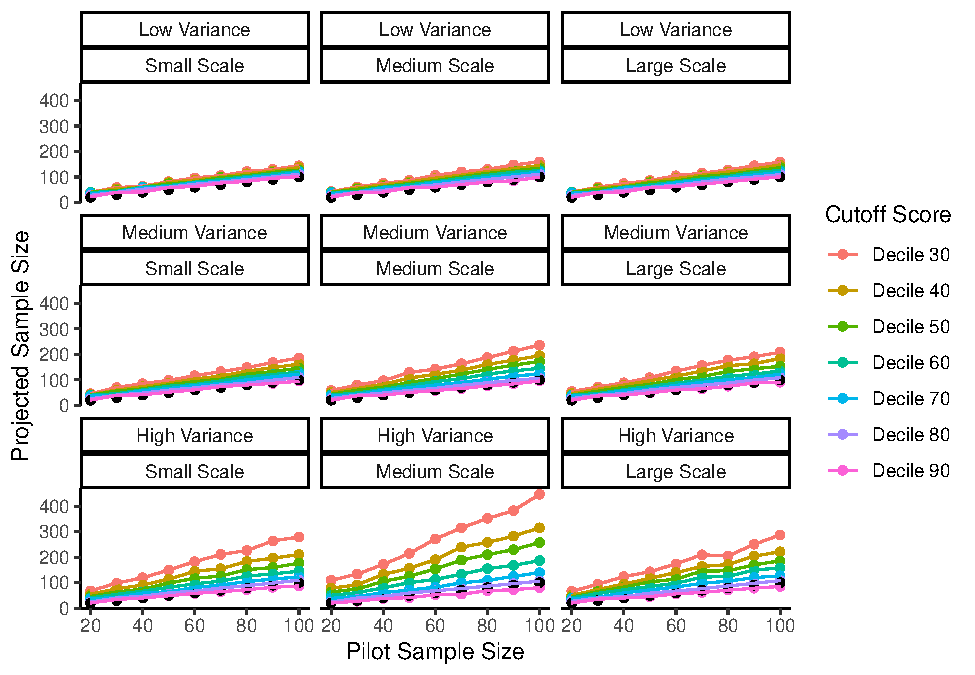
\includegraphics{manuscript_draft_files/figure-latex/item-figure-1.pdf}
\caption{\label{fig:item-figure}Add a good caption here.}
\end{figure}

\hypertarget{projected-sample-size-sensitivity-to-pilot-sample-size}{%
\subsection{Projected Sample Size Sensitivity to Pilot Sample Size}\label{projected-sample-size-sensitivity-to-pilot-sample-size}}

In our second question, we examined if the suggested procedure was sensitive to the amount of information present in the pilot data. Larger pilot data is more informative, and therefore, we should expect a lower projected sample size. As shown in Figure \ref{fig:sensitive-figure} for only the low variability and small scale data, we do not find this effect. These simulations from the pilot data would nearly always suggest a larger sample size - mostly in a linear trend increasing with sample sizes. This result comes from the nature of the procedure - if we base our estimates on a SE cutoff, we will almost always need a bit more people for items to meet those goals. This result does not achieve our second goal.

\begin{figure}
\centering
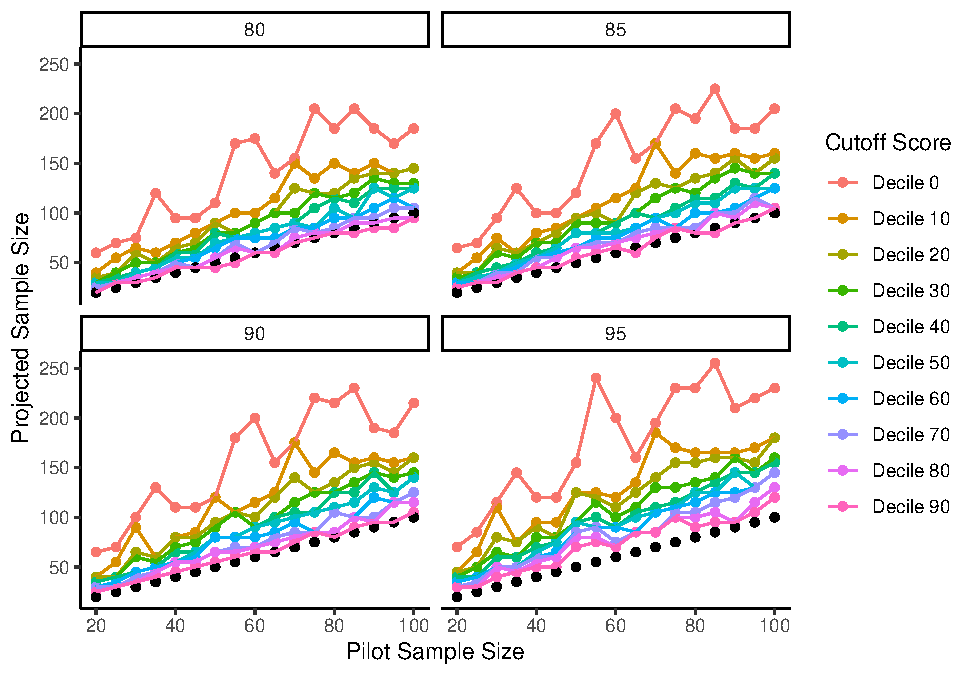
\includegraphics{manuscript_draft_files/figure-latex/sensitive-figure-1.pdf}
\caption{\label{fig:sensitive-figure}Add good description here.}
\end{figure}

Therefore, we suggest using a correction factor on the simulation procedure to account for the known asymptotic nature of power (i.e., at larger sample sizes power increases level off). For this function in our simulation study, we combined a correction factor for upward biasing of effect sizes (Hedges' correction) with the formula for exponential decay calculations. The decay factor was calculated as follows:

\[ 1 - \sqrt{\frac{N_{Pilot} - min(N_{Simulation})}{N_{Pilot}}}^{log_2(N_{Pilot})}\]

\(N_{Pilot}\) indicates the sample size of the pilot data minus the minimum simulated sample size to ensure that the smallest sample sizes do not decay (i.e., the formula zeroes out). This value is raised to the power of \(log_2\) of the sample size of the pilot data, which decreases the impact of the decay to smaller increments for increasing sample sizes. This value is then multiplied by the projected sample size. As shown in Figure \ref{fig:corrected-figure}, this correction factor produces the desired quality of maintaining that small pilot studies should \emph{increase} sample size, and that sample size suggestions level off as pilot study data sample size increases.

\begin{figure}
\centering
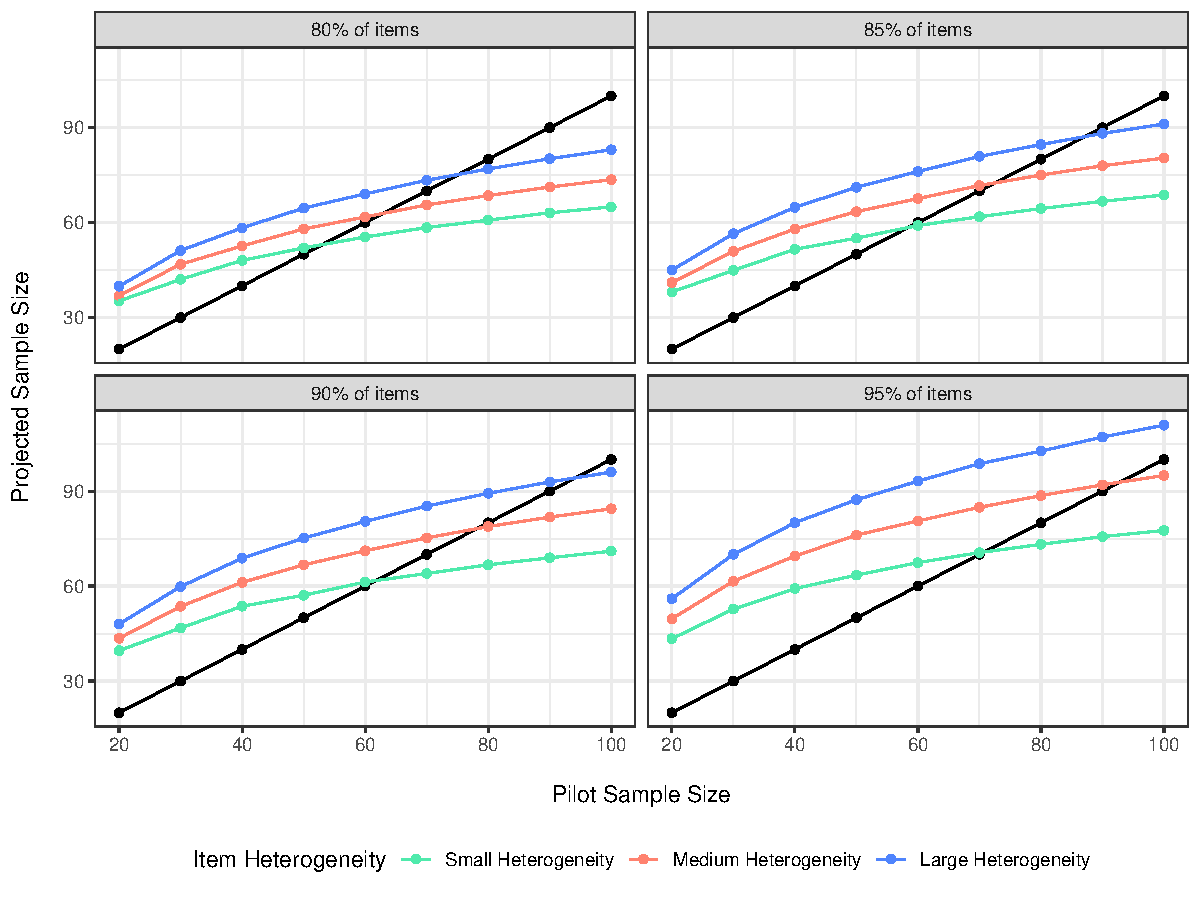
\includegraphics{manuscript_draft_files/figure-latex/corrected-figure-1.pdf}
\caption{\label{fig:corrected-figure}A corrected figure update this caption.}
\end{figure}

\hypertarget{corrections-for-individual-researchers}{%
\subsection{Corrections for Individual Researchers}\label{corrections-for-individual-researchers}}

We have portrayed that this procedure, with a correction factor, can perform as desired. However, within real scenarios, researchers will only have one pilot sample, not the various simulated samples shown above. What should the researcher do to correct their projected sample size from their own pilot data simulations?

To explore if we could recover the new projected sample size from data a researcher would have, we used linear models to create a formula for researcher correction. First, the corrected projected sample size was predicted by the original projected sample size. Next, the standard deviation of the item standard deviations was added to the equation to recreate heterogeneity estimates. The scale of the data is embedded into the standard deviation of the items (\emph{r} = 0.80), and therefore, this variable was not included separately. Last, we included the pilot sample size.

The first model using pilot sample size to predict new sample size was significant, \emph{F}(1, 2266) = 23,280.26, \emph{p} \textless{} .001, \(R^2 = .91\), 90\% CI \([0.91, 0.92]\), capturing nearly 90\% of the variance, \(b = 0.53\), 95\% CI \([0.52, 0.54]\). The second model with item standard deviation was better than the first model \emph{F}(1, NULL) = 13.59, \emph{p} \textless{} .001, \(R^2 = .91\), 90\% CI \([0.91, 0.92]\). The item standard deviation predictor was significant, \(b = 0.01\), 95\% CI \([0.00, 0.02]\), \(t(2265) = 2.20\), \(p = .028\). The addition of the original pilot sample size was also significant, \emph{F}(1, NULL) = 4,101.10, \emph{p} \textless{} .001, \(R^2 = .97\), 90\% CI \([0.97, 0.97]\).

As shown in the final model Table \ref{tab:table-correction}, the new suggested sample size is proportional to the original suggested sample size (i.e., \emph{b} \textless{} 1), which reduces the sample size suggestion. As variability increases, the suggested sample size also increases to capture differences in heterogeneity shown above; however, this predictor is not significant in the final model, and only contributes a small portion of overall variance. Last, in order to correct for large pilot data, the original pilot sample size decreases the new suggested sample size. This formula approximation captures 96\% of the variance in sample size scores and should allow a researcher to estimate based on their own data.

\begin{table}[tbp]

\begin{center}
\begin{threeparttable}

\caption{\label{tab:table-correction}Parameters for All Decile Cutoff Scores}

\begin{tabular}{lllll}
\toprule
Term & Estimate & $SD$ & $t$ & $p$\\
\midrule
Intercept & 34.549 & 0.425 & 81.264 & < .001\\
Projected Sample Size & 0.621 & 0.003 & 247.039 & < .001\\
Item SD & 0.000 & 0.003 & 0.014 & .989\\
Pilot Sample Size & -0.483 & 0.008 & -64.040 & < .001\\
\bottomrule
\end{tabular}

\end{threeparttable}
\end{center}

\end{table}

\hypertarget{choosing-an-appropriate-cutoff}{%
\subsection{Choosing an Appropriate Cutoff}\label{choosing-an-appropriate-cutoff}}

Last, we examine the question of an appropriate SE decile. All graphs for power, heterogeneity, scale, and correction are presented online. First, the 0\%, 10\%, and 20\% deciles are likely too restrictive, providing very large estimates that do not always find a reasonable sample size in proportion to the pilot sample size, scale, and heterogeneity. If we examine the \(R^2\) values for each decile of our regression equation separately, we find that the 50\% (0.97) represents the best match to our corrected sample size suggestions. The 50\% decile, in the corrected format, appears to meet all goals: 1) increases with heterogeneity and scale of data, and 2) higher suggested values for small original samples and a leveling effect at larger pilot data. Figure \ref{fig:decile-figure} illustrates the corrected scores for simulations at the 50\% decile recommended cutoff for item standard errors.

\begin{figure}
\centering
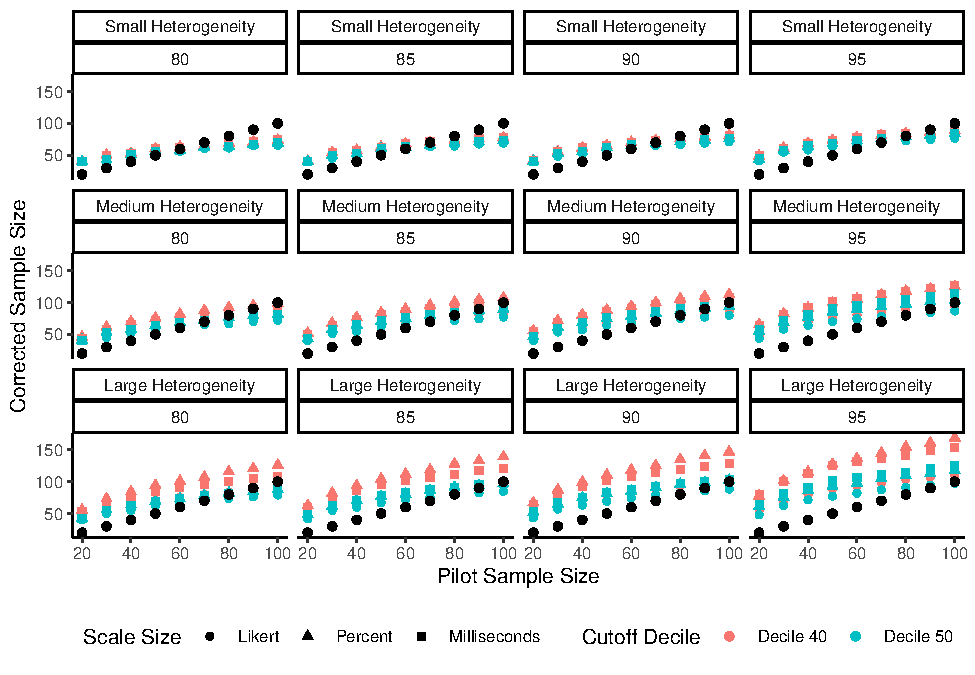
\includegraphics{manuscript_draft_files/figure-latex/decile-figure-1.pdf}
\caption{\label{fig:decile-figure}A picture of the 50\% cutoff.}
\end{figure}

The formula for finding the corrected sample size using a 50\% decile is: \(N_{Corrected Projected} = 39.269 + 0.700 \times X_{N_{Projected}} + 0.003 \times X_{SD Items} - 0.694 \times X_{N_{Pilot}}\). The suggested sample size will be estimated from the 80\%, 85\%, 90\%, or 95\% selection at the 50\% decile as shown above. The item SD can be calculated directly from the data, and the pilot sample size is the sample size of the data from which a researcher is simulating their samples. Therefore, we will recommend the 50\% decile of the item standard errors for step 2 of our suggested simulation procedure, and to correct the projected sample sizes found in step 5 using the correction equation above. While the estimated coefficients could change given variations on our simulation parameters, the general size and pattern of coefficients was consistent, and therefore, we believe this correction equation should work for a variety of use cases.

\hypertarget{examples}{%
\section{Examples}\label{examples}}

In this section, we provide two examples of the suggested procedure. The first example includes concreteness ratings from Brysbaert, Warriner, and Kuperman (2014). Instructions given to participants denoted the difference between concrete (i.e., ``refers to something that exists in reality'') and abstract (i.e., ``something you cannot experience directly through your senses or actions'') terms. Participants were then asked to rate concreteness of terms using a 1 (abstract) to 5 (concrete) scale. This data represents a small scale dataset that could be used as pilot data for a study using concrete word ratings. The data is available at \url{https://osf.io/qpmf4/}. The second dataset includes a large scale dataset with response latencies, the English Lexicon Project (Balota et al., 2007). The English Lexicon Project consists of lexical decision response latencies for English words. In a lexical decision task, participants simply select ``word'' for real words (e.g., \emph{dog}) and ``nonword'' for pseudowords (e.g., \emph{wug}). The trial level data is available here {[}\url{https://elexicon.wustl.edu/}{]}. Critically, in each of these examples, the individual trial level data for each item is available to simulate and calculate standard errors on. Data that has been summarized could potentially be used, as long as the original standard deviations for each item were present. From the mean and standard deviation for each item, a simulated pilot dataset could be generated for estimating new sample sizes. All code to estimate sample sizes is provided on our OSF page.

\hypertarget{concreteness-ratings}{%
\subsection{Concreteness Ratings}\label{concreteness-ratings}}

The concreteness ratings data includes 63039 concepts that were rated for their concreteness. In our fictional study for this example, we selected 100 random words to show participants. In the original study, not every participant rated every word, which created uneven sample sizes for each word. In our random sample of 100 words, the average pilot sample size was 28.15 (\emph{SD} = 1.59), and we will use 28 as our pilot sample size for this example. All ``do not know'' ratings were set as missing data. The 50\% decile for items standard error was 0.25 for our cutoff criterion.

The pilot data was then simulated, with replacement, with samples from 20 to 300 increasing in units of 5. On each sample, the percent of items below the cutoff score were calculated. After applying our correction equation, we find that a sample size of 44 would allow for at least 80\% of items to meet the cutoff criterion. The sample sizes for 85\% (48), 90\% (48), and 95\% (51) are also options for sample size suggestions. Finally, we calculated the potential amount of data retention given that participants could indicate they did not know a word (\(M_{correct}\) = 0.79, \emph{SD} = 0.24). In order to account for this facet, the potential sample sizes were multiplied by 1/0.79, which results in a suggested sample of 56, 61, and 65. Therefore, we could designate our minimum sample per item as 56, stopping rule of 0.25, and maximum sample size of 65.

\hypertarget{response-latencies}{%
\subsection{Response Latencies}\label{response-latencies}}

The ELP response latency data includes 80962 word-forms, 40481 that are listed as non-words, and 40481 real words. For our example study, we will randomly select 500 real words and 500 non-words to show participants. The average pilot sample size for this random sample was 32.72 (\emph{SD} = 0.64), and \emph{n} = 33 will be our pilot size for this example. Again, participants are expected to make mistakes, and we calculated percent correct as 0.85, which was roughly even in the two stimulus categories: \(M_{word}\) = 0.82 and \(M_{non-word}\) = 0.88. The 50\% decile for items standard error was 61.23 for our cutoff criterion. We additionally checked to ensure that the two stimulus types did not have very different cutoff criterions: 50\% decile \(SE_{words}\) = 58.98, 50\% decile \(SE_{nonwords}\) = 62.61. In this scenario, we could choose to go with the lower SE to be more conservative (i.e., higher projected sample size). Given the values were close for large scale data, we used the 50\% decile of all stimuli taken together.

The pilot response latency data was then simulated in the same way as described above. After calculating the percent below our cutoff score, we applied the correction to the projected sample sizes. A sample size of 31 would equate to 80\% of the items reaching our cutoff, along with 85\% (34), 90\% (34), and 95\% (38). Again, we adjusted for data loss given that participants are expected to incorrectly answer items, resulting in a suggested sample of 36, 40, and 45. One other possible consideration for this study is potential fatigue in showing participants 1000 target items. Therefore, we could designate in our research design that each participant will only receive 500 of the target items. We would need to double our sample sizes to account for splitting of the items across multiple sets of participants. Our minimum sample size for the entire study could be 72, stopping rule of 61.23, and maximum sample size of 90. This study would benefit from an adaptive design, where smaller sets items are randomly sampled for participants until they reach the minimum sample size or the cutoff criteria. At this point, items are probabilistically sampled (e.g., higher selection probability for items that have not reached a minimum or stopping rule) until all items have reached criteria.

\hypertarget{additional-materials}{%
\subsection{Additional Materials}\label{additional-materials}}

While the examples in this manuscript are traditionally cognitive linguistics focused, any research using repeated items can benefit from newer sampling techniques. Therefore, we provide XX example vignettes and code examples on our OSF page/GitHub site for this manuscript across a range of examples of data types provided by the authors of this manuscript. Examples include psycholinguistics, social psychology, COVID related data, and cognitive psychology.

\hypertarget{discussion}{%
\section{Discussion}\label{discussion}}

In this manuscript, we demonstrated a method using AIPE and simulation/bootstrapping to estimate a minimum and maximum sample size along with a rule for stopping data collection based on narrow confidence intervals on the parameter of interest. We believe this procedure is specifically useful for studies with multiple items that intend on using item level focused analyses; however, the utility of measuring each item well can extend to many analysis choices. By focusing on gathering quality data, we can suggest that the data is useful, regardless of outcome of any hypothesis test.

One limitation of these methods would be using datasets with very large numbers of items to simulate what might happen within one study. For example, the English Lexicon Project includes thousands of items, and by the time we would simulate for all of those, it would likely suggest needing thousands of participants for \emph{most items} to reach criterion. Alternatively, as the number of items increases, you also could potentially see very small estimates for sample size due to the correction factor (as with large numbers of items, you could find many items with standard errors below the 50\% decile). Therefore, it would be beneficial to consider only simulating with what a participant would reasonably complete in a study. On the other side, small numbers of repeated items usually result in higher sample sizes proposed from the original pilot data. This result occurs because the smaller number of items means more samples for nearly all to reach the cutoff criteria. These results are not too different than what we might expect for a power analysis using a multilevel model - larger number of items tends to decrease necessary sample size, while smaller numbers of items tend to increase sample size.

Second, these methods do not ensure the normal interpretation of power, wherein you know would find a specific effect for a specific test, \(\alpha\), and so on. As discussed in the introduction, there is not necessarily a one-to-one mapping of hypothesis to analysis, and many of the guesses within a traditional power analysis are just that - best guesses for various parameters. These methods could be used together to strengthen our understanding of sample size necessary for both a hypothesis test and well tuned estimation.

\newpage

\hypertarget{references}{%
\section{References}\label{references}}

\begingroup
\setlength{\parindent}{-0.5in}
\setlength{\leftskip}{0.5in}

\hypertarget{refs}{}
\begin{CSLReferences}{1}{0}
\leavevmode\vadjust pre{\hypertarget{ref-anderson2017}{}}%
Anderson, S. F., Kelley, K., \& Maxwell, S. E. (2017). Sample-Size Planning for More Accurate Statistical Power: A Method Adjusting Sample Effect Sizes for Publication Bias and Uncertainty. \emph{Psychological Science}, \emph{28}(11), 1547--1562. \url{https://doi.org/10.1177/0956797617723724}

\leavevmode\vadjust pre{\hypertarget{ref-balota2007}{}}%
Balota, D. A., Yap, M. J., Hutchison, K. A., Cortese, M. J., Kessler, B., Loftis, B., \ldots{} Treiman, R. (2007). The English Lexicon Project. \emph{Behavior Research Methods}, \emph{39}(3), 445--459. \url{https://doi.org/10.3758/BF03193014}

\leavevmode\vadjust pre{\hypertarget{ref-batterham2005}{}}%
Batterham, A. M., \& Atkinson, G. (2005). How big does my sample need to be? A primer on the murky world of sample size estimation. \emph{Physical Therapy in Sport}, \emph{6}(3), 153--163. \url{https://doi.org/10.1016/j.ptsp.2005.05.004}

\leavevmode\vadjust pre{\hypertarget{ref-beribisky2019}{}}%
Beribisky, N. (2019). \emph{A Multi-Faceted Mess: A Review of Statistical Power Analysis in Psychology Journal Articles}. Retrieved from \url{https://yorkspace.library.yorku.ca/xmlui/handle/10315/36719}

\leavevmode\vadjust pre{\hypertarget{ref-brysbaert2018}{}}%
Brysbaert, M., \& Stevens, M. (2018). Power Analysis and Effect Size in Mixed Effects Models: A Tutorial. \emph{Journal of Cognition}, \emph{1}(1), 9. \url{https://doi.org/10.5334/joc.10}

\leavevmode\vadjust pre{\hypertarget{ref-brysbaert2014}{}}%
Brysbaert, M., Warriner, A. B., \& Kuperman, V. (2014). Concreteness ratings for 40 thousand generally known English word lemmas. \emph{Behavior Research Methods}, \emph{46}(3), 904--911. \url{https://doi.org/10.3758/s13428-013-0403-5}

\leavevmode\vadjust pre{\hypertarget{ref-buchanan2019}{}}%
Buchanan, E. M., Valentine, K. D., \& Maxwell, N. P. (2019). LAB: Linguistic Annotated Bibliography {\textendash} a searchable portal for normed database information. \emph{Behavior Research Methods}, \emph{51}(4), 1878--1888. \url{https://doi.org/10.3758/s13428-018-1130-8}

\leavevmode\vadjust pre{\hypertarget{ref-chalmers2020}{}}%
Chalmers, R. P., \& Adkins, M. C. (2020). Writing effective and reliable monte carlo simulations with the SimDesign package. \emph{The Quantitative Methods for Psychology}, \emph{16}(4), 248--280. \url{https://doi.org/10.20982/tqmp.16.4.p248}

\leavevmode\vadjust pre{\hypertarget{ref-champely2017}{}}%
Champely, S., Ekstrom, C., Dalgaard, P., Gill, J., Weibelzahl, S., Anandkumar, A., \ldots{} De Rosario, H. (2017). \emph{Pwr: Basic functions for power analysis}.

\leavevmode\vadjust pre{\hypertarget{ref-cohen1990}{}}%
Cohen, J. (1990). Things I have learned (so far). \emph{American Psychologist}, \emph{45}(12), 1304--1312. \url{https://doi.org/10.1037/0003-066X.45.12.1304}

\leavevmode\vadjust pre{\hypertarget{ref-coretta}{}}%
Coretta, S., Casillas, J., {[}participating authors{]}, \& Roettger, T. B. (n.d.). Multidimensional signals and analytic flexibility: Estimating degrees of freedom in human speech analyses. \emph{Advances in Methods and Practices in Psychological Science}.

\leavevmode\vadjust pre{\hypertarget{ref-d.chambers2014}{}}%
D. Chambers, C., Feredoes, E., D. Muthukumaraswamy, S., J. Etchells, P., \& 1 Cardiff University Brain Research Imaging Centre, School of Psychology, Cardiff University; (2014). Instead of {``}playing the game{''} it is time to change the rules: Registered Reports at AIMS Neuroscience and beyond. \emph{AIMS Neuroscience}, \emph{1}(1), 4--17. \url{https://doi.org/10.3934/Neuroscience.2014.1.4}

\leavevmode\vadjust pre{\hypertarget{ref-debruine2021}{}}%
DeBruine, L. (2021). \emph{Faux: Simulation for factorial designs}. Zenodo. \url{https://doi.org/10.5281/ZENODO.2669586}

\leavevmode\vadjust pre{\hypertarget{ref-erdfelder1996}{}}%
Erdfelder, E., Faul, F., \& Buchner, A. (1996). GPOWER: A general power analysis program. \emph{Behavior Research Methods, Instruments, \& Computers}, \emph{28}(1), 1--11. \url{https://doi.org/10.3758/BF03203630}

\leavevmode\vadjust pre{\hypertarget{ref-faul2007}{}}%
Faul, F., Erdfelder, E., Lang, A.-G., \& Buchner, A. (2007). G*Power 3: A flexible statistical power analysis program for the social, behavioral, and biomedical sciences. \emph{Behavior Research Methods}, \emph{39}(2), 175--191. \url{https://doi.org/10.3758/BF03193146}

\leavevmode\vadjust pre{\hypertarget{ref-halpern2002}{}}%
Halpern, S. D. (2002). The Continuing Unethical Conduct of Underpowered Clinical Trials. \emph{JAMA}, \emph{288}(3), 358. \url{https://doi.org/10.1001/jama.288.3.358}

\leavevmode\vadjust pre{\hypertarget{ref-doi:10.1177ux2f1745691620979806}{}}%
Hardwicke, T. E., Thibault, R. T., Kosie, J. E., Wallach, J. D., Kidwell, M. C., \& Ioannidis, J. P. A. (2022). Estimating the prevalence of transparency and reproducibility-related research practices in psychology (2014{\textendash}2017). \emph{Perspectives on Psychological Science}, \emph{17}(1), 239--251. \url{https://doi.org/10.1177/1745691620979806}

\leavevmode\vadjust pre{\hypertarget{ref-hardwicke2020}{}}%
Hardwicke, T. E., Wallach, J. D., Kidwell, M. C., Bendixen, T., Crüwell, S., \& Ioannidis, J. P. A. (2020). An empirical assessment of transparency and reproducibility-related research practices in the social sciences (2014{\textendash}2017). \emph{Royal Society Open Science}, \emph{7}(2), 190806. \url{https://doi.org/10.1098/rsos.190806}

\leavevmode\vadjust pre{\hypertarget{ref-kelley2007}{}}%
Kelley, K. (2007). Sample size planning for the coefficient of variation from the accuracy in parameter estimation approach. \emph{Behavior Research Methods}, \emph{39}(4), 755--766. \url{https://doi.org/10.3758/BF03192966}

\leavevmode\vadjust pre{\hypertarget{ref-maxwell2008}{}}%
Maxwell, S. E., Kelley, K., \& Rausch, J. R. (2008). Sample size planning for statistical power and accuracy in parameter estimation. \emph{Annual Review of Psychology}, \emph{59}, 537--563. \url{https://doi.org/10.1146/annurev.psych.59.103006.093735}

\leavevmode\vadjust pre{\hypertarget{ref-nosek2014}{}}%
Nosek, B. A., \& Lakens, D. (2014). Registered Reports: A Method to Increase the Credibility of Published Results. \emph{Social Psychology}, \emph{45}(3), 137--141. \url{https://doi.org/10.1027/1864-9335/a000192}

\leavevmode\vadjust pre{\hypertarget{ref-nuijten2016}{}}%
Nuijten, M. B., Hartgerink, C. H. J., Assen, M. A. L. M. van, Epskamp, S., \& Wicherts, J. M. (2016). The prevalence of statistical reporting errors in psychology (1985{\textendash}2013). \emph{Behavior Research Methods}, \emph{48}(4), 1205--1226. \url{https://doi.org/10.3758/s13428-015-0664-2}

\leavevmode\vadjust pre{\hypertarget{ref-opensciencecollaboration2015}{}}%
Open Science Collaboration. (2015). Estimating the reproducibility of psychological science. \emph{Science}, \emph{349}(6251), aac4716--aac4716. \url{https://doi.org/10.1126/science.aac4716}

\leavevmode\vadjust pre{\hypertarget{ref-rosenthal1979}{}}%
Rosenthal, R. (1979). The file drawer problem and tolerance for null results. \emph{Psychological Bulletin}, \emph{86}(3), 638--641. \url{https://doi.org/10.1037/0033-2909.86.3.638}

\leavevmode\vadjust pre{\hypertarget{ref-rousselet}{}}%
Rousselet, G., Pernet, D. C., \& Wilcox, R. R. (n.d.). \emph{An introduction to the bootstrap: A versatile method to make inferences by using data-driven simulations}. \url{https://doi.org/10.31234/osf.io/h8ft7}

\leavevmode\vadjust pre{\hypertarget{ref-silberzahn2018many}{}}%
Silberzahn, R., Uhlmann, E. L., Martin, D. P., Anselmi, P., Aust, F., Awtrey, E., \ldots{} others. (2018). Many analysts, one data set: Making transparent how variations in analytic choices affect results. \emph{Advances in Methods and Practices in Psychological Science}, \emph{1}(3), 337356.

\leavevmode\vadjust pre{\hypertarget{ref-simmons2011}{}}%
Simmons, J. P., Nelson, L. D., \& Simonsohn, U. (2011). False-positive psychology: Undisclosed flexibility in data collection and analysis allows presenting anything as significant. \emph{Psychological Science}, \emph{22}(11), 1359--1366. \url{https://doi.org/10.1177/0956797611417632}

\leavevmode\vadjust pre{\hypertarget{ref-stewart2020}{}}%
Stewart, S., Rinke, E. M., McGarrigle, R., Lynott, D., Lunny, C., Lautarescu, A., \ldots{} Crook, Z. (2020). \emph{Pre-registration and registered reports: A primer from UKRN}. \url{https://doi.org/10.31219/osf.io/8v2n7}

\leavevmode\vadjust pre{\hypertarget{ref-vazire2018}{}}%
Vazire, S. (2018). Implications of the Credibility Revolution for Productivity, Creativity, and Progress. \emph{Perspectives on Psychological Science}, \emph{13}(4), 411--417. \url{https://doi.org/10.1177/1745691617751884}

\leavevmode\vadjust pre{\hypertarget{ref-williamson2000}{}}%
Williamson, P., Hutton, J. L., Bliss, J., Blunt, J., Campbell, M. J., \& Nicholson, R. (2000). Statistical review by research ethics committees. \emph{Journal of the Royal Statistical Society: Series A (Statistics in Society)}, \emph{163}(1), 5--13. \url{https://doi.org/10.1111/1467-985X.00152}

\end{CSLReferences}

\endgroup


\end{document}
